\chapter{Reducing uncertainty in high-throughput microarray studies}
\label{ch:preproc} 

\begin{quotation}
  \emph{As far as the laws of mathematics refer to reality, they are
    not certain, as far as they are certain, they do not refer to
    reality.}
\begin{flushright}
%\citep{Einstein56}
A. Einstein (1956)
\end{flushright}
\end{quotation}

Gene expression microarrays are currently the most widely used
technology for genome-wide transcriptional profiling, and they
constitute the main source of data in this thesis. An overview of
microarray technology is provided in
Section~\ref{sec:biodata}. Microarray measurements are associated with
high levels of noise from technical and biological
sources. Appropriate preprocessing techniques can help to reduce noise
and obtain reliable measurements, which is the crucial starting point
for any data analysis task. This chapter presents the first main
contribution of the thesis, preprocessing techniques that utilize side
information in genomic sequence databases and microarray data collections in order to improve the accuracy
of high-throughput gene expression data. The chapter is organized as follows: Section~\ref{sec:noise} gives an overview of the various sources of noise in high-throughput microarray studies. Section~\ref{sec:preprocessing} introduces a strategy for noise reduction based on side information in external genomic sequence databases. Section~\ref{sec:modelnoise} extends this model by describing a model-based approach that additionally combines statistical evidence across multiple microarray experiments in order to provide quantitative information of probe performance and utilizes this information to improve the reliability of high-throughput observations. The results are summarized in Section~\ref{sec:preconclusion}.


\section{Sources of uncertainty}\label{sec:noise}

Measurement data obtained with novel high-throughput technologies
comes with high levels of uncontrolled biological and technical
variation. This is often called {\it noise} as it obscures the
measurements, and adds potential bias and variance on the {\it signal}
of interest. Biological noise is associated with natural biological
variation between cell populations, cellular processes and
individuals.  Single-nucleotide polymorphisms, alternative splicing
and non-specific hybridization add biological variation in the data
\citep{Dai05,Zhang05}. More technical sources of noise in the
measurement process include RNA extraction and amplification,
experiment-specific variation, as well as platform- and
laboratory-specific effects \citep{Choi03, Shi06,Tu02}.


A significant source of noise on gene expression arrays comes from
individual probes that are designed to measure the activity of a given
transcript in a biological sample. Figure~\ref{fig:badprobe}A
shows probe-level observations of differential gene expression for a
collection of probes designed to target the same mRNA transcript. One
of the probes is highly contaminated and likely to add unrelated
variation to the analysis. A number of factors affect probe
performance.  For instance, it has been reported in
Publication~\ref{PECA} and elsewhere \citep{Hwang04,Mecham04b} that a
large portion of microarray probes may target unintended mRNA
sequences. Moreover, although the probes have been designed to
uniquely hybridize with their intended mRNA target, remarkable
cross-hybridization with the probes by single-nucleotide polymorphisms
\citep{Dai05, Sliwerska07} and other mRNAs with closely similar
sequences \citep{Zhang05} have been reported; high-affinity probes
with high GC-content may have higher likelihood of cross-hybridization
with nonspecific targets \citep{Mei03}.  Alternative splicing
\citep{Shi06} and mRNA degradation \citep{Auer03} may cause
differences between probes targeting different positions of the gene
sequence. Such effects will contribute to probe-level contamination in
a probe- and condition-specific manner. However, sources of
probe-level noise are still poorly understood \citep{Irizarry05,Li05}
despite their importance for expression analysis and probe design.

High levels of noise set specific challenges for analysis. Better
understanding of the technical aspects of the measurement process will
lead to improved analytical procedures and ultimately to more
accurate biological results \citep{Reimers2010}. Publication~\ref{RPA}
provides computational tools to investigate probe performance and the
relative contributions of the various sources of probe-level
contamination on short oligonucleotide arrays.

\begin{figure}[t]
\label{fig:badprobe}
\begin{center}
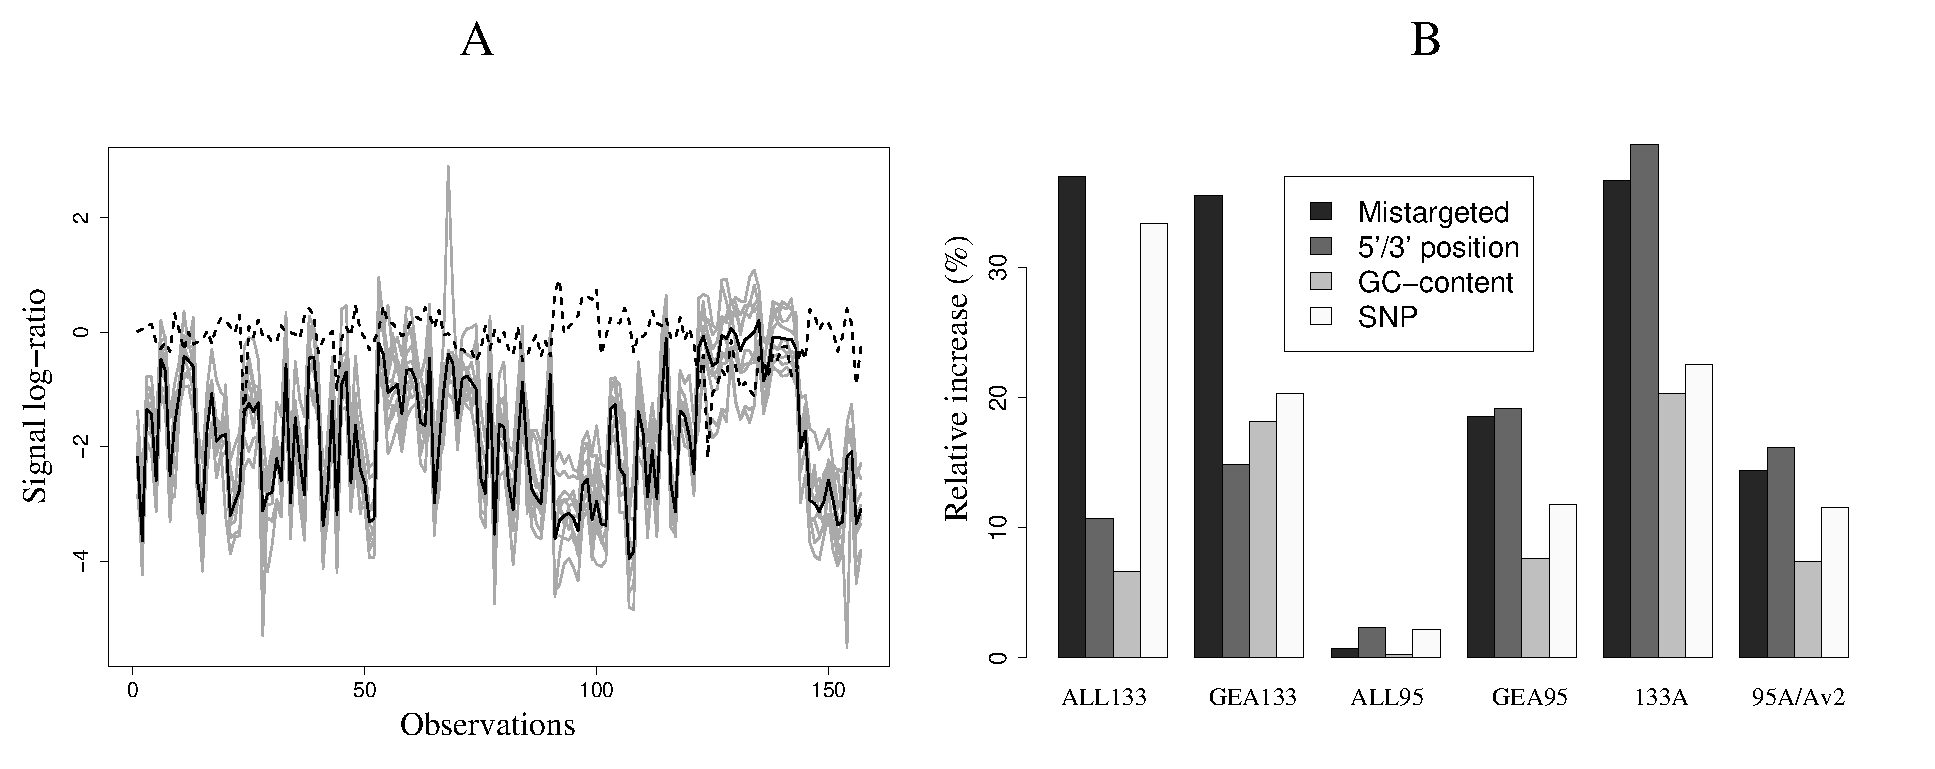
\includegraphics[width=\textwidth]{pic/probecomparison.eps}
\end{center}
\caption{{\bf A} Example of a probe set that contains a probe with
  high contamination levels (dashed line) detected by the
  probabilistic RPA model. The probe-level observations of
  differential gene expression for the different probes that measure
  the same target transcript are indicated by gray lines. The black
  line shows the estimated signal of the target transcript across a
  number of conditions. {\bf B} Increase in the average variance of
  the probes associated with the investigated noise sources:
  mistargeted probes having errors in the genomic alignment, most
  5'/3' probes of each probe set, GC-rich, and SNP-associated probes.
  The variances were estimated by RPA and describe the noise level of
  the probes. The results are shown for the individual ALL and GEA
  data sets, and for their combined results on both platforms (133A
  and 95A/Av2). \copyright IEEE. Reprinted with permission from
  Publication~\ref{RPA}.} %[FIXME pitaako mainita IEEE]
\end{figure}
%See /share/mi/exp/RBA07/EMimplementation/validation
%/share/mi/exp/RBA07/EMimplementation/validation/ 215157_x_atB.eps
% produced with 
%/share/mi/exp/RBA07/EMimplementation/validation/probesetFigure2.R

\section{Preprocessing microarray data with side
  information}\label{sec:preprocessing}

{\it Preprocessing} of the {\it raw data} obtained from the original
measurements can help to reduce noise and improve comparability
between microarray experiments. Preprocessing can be defined in terms
of statistical transformations on the raw data, and this is a central
part of data analysis in high-throughput studies. This section
outlines the standard preprocessing steps for short oligonucleotide
arrays, the main source of transcriptional profiling data in this
thesis. However, the general concepts also apply to other microarray
platforms \citep{Reimers2010}.

\subsubsection{Standard preprocessing steps}

A number of preprocessing techniques for short oligonucleotide arrays
have been introduced \citep{Irizarry06, Reimers2010}. The standard
preprocessing steps in microarray analysis include quality control,
background correction, normalization and summarization.

{\it Microarray quality control} is used to identify arrays with
remarkable experimental defects, and to remove them from subsequent
analysis. The typical tests consider RNA degradation levels and a
number of other summary statistics to guarantee that the array data is
of reasonable quality. The arrays that pass the microarray quality
control are preprocessed further. Each array typically has spatial
biases that vary smoothly across the array, arising from technical
factors in the experiment. {\it Background correction} is used to
detect and remove such spatial effects from the array data, and to
provide a uniform background signal, enhancing the comparability of
the probe-level observations between different parts of the
array. Moreover, background correction can estimate the general noise
level on the array; this helps to detect probes whose signal differs
significantly from the background noise. Robust multi-array averaging
(RMA) is one of the most widely used approaches for preprocessing
short oligonucleotide array data \citep{Irizarry03rma}.  The
background correction in RMA is based on a global model for probe
intensities. The observed intensity, \(Y\), is modeled as a sum of an
exponential signal component, \(S\) and Gaussian noise
\(B\). Background corrected data is then obtained as the expectation
\(\E_B(S|Y)\). While background correction makes the observations
comparable within array, {\it normalization} is used to improve the
comparability between arrays. Quantile normalization is a widely used
method that forces all arrays to follow the same empirical intensity
distribution \citep[see e.g.][]{Bolstad03}.  Quantile normalization
makes the measurements across different arrays comparable, assuming
that the overall distribution of mRNA concentration is approximately
the same in all cell populations. This has proven to be a feasible
assumption in transcriptional profiling studies. As always, there are
exceptions. For instance, human brain tissues have systematic
differences in gene expression compared to other organs. On short
oligonucleotide arrays, a number of probes target the same
transcript. In the final {\it summarization step}, the individual
probe-level observations of each target transcript are summarized into
a single summary estimate of transcript activity. Standard algorithmic
implementations are available for each preprocessing step.


\subsubsection{Probe-level preprocessing methods}

Differences in probe characteristics cause systematic differences in
probe performance.  The use of several probes for each target leads to
more robust estimates on transcript activity but it is clear that
probe quality may significantly affect the results of a microarray
study \citep{Irizarry03}. Widely used preprocessing algorithms utilize
probe-specific parameters to model probe-specific effects in the probe
summarization step. Some of the first and most well-known probe-level 
preprocessing algorithms include dChip/MBEI \citep{Li01mbei}, RMA \citep{Irizarry03rma}, and
gMOS \citep{Milo03}. Taking probe-level effects into account can
considerably improve the quality of a microarray study
\citep{Reimers2010}. Publications~\ref{PECA} and~\ref{RPA} incorporate
side information of the probes to preprocessing, and introduce
improved probe-level analysis methods for differential gene expression
studies.

In order to introduce probe-level preprocessing methods in more
detail, let us consider the probe summarization step of the RMA
algorithm \citep{Irizarry03rma}. RMA has a Gaussian model for probe
effects with probe-specific mean parameters and a shared variance
parameter for the probes.  The mean parameters characterize
probe-specific binding affinities that cause systematic differences in
the signal levels captured by each probe. Estimating the
probe-specific effects helps to remove this effect in the final
probeset-level summary of the probe-level observations. To briefly
outline the algorithm, let us consider a collection of probes (a {\it
  probeset}) that measure the expression level of the same target
transcript \(g\) in condition \(i\). The probe-level observations are
modeled as a sum of the true, underlying expression signal \(\gi\),
which is common to all probes, probe-specific binding affinity
\(\muj\), and Gaussian noise \(\epsilon\). A probe-level observation
for probe \(j\) in condition \(i\) is then modeled in RMA as

\begin{equation}\label{eq:rmamodel}
  \sij = \gi + \muj + \epsilon.
\end{equation} 

Measurements from multiple conditions are needed to estimate the
probe-specific effects \(\muj\). RMA and other models that measure
absolute gene expression have an important drawback: the probe
affinity effects \(\{\muj\}\) are unidentifiable. In order to obtain
an identifiable model, the RMA algorithm includes an additional
constraint that the probe affinity effects are zero on average:
\(\Sigma_j\muj = 0\). This yields a well-defined algorithm that has
been shown to produce accurate measurements of gene expression in
practical settings. Further extensions of the RMA algorithm include
gcRMA, which has a more detailed chemical model for the probe effects
\citep{Wu04}, refRMA \citep{Katz06}, which utilizes probe-specific
effects derived from background data collections, and fRMA
\citep{McCall2010}, which also models batch-specific effects in
microarray studies. The estimation of unidentifiable probe affinities
is a main challenge for most probe-level preprocessing models.

RMA and other probe-level models for short oligonucleotide arrays have
been designed to estimate absolute expression levels of the
genes. However, gene expression studies are often ultimately targeted
at investigating {\it differential expression levels}, that is,
differences in gene expression between experimental conditions.
Measurements of differential expression is obtained for instance by
comparing the expression levels, obtained through the RMA algorithm or
other methods, between different conditions.  However, the
summarization of the probe-level values is then performed prior to the
actual comparison. Due to the unidentifiability of the probe affinity
parameters in the RMA and other probe-level models, this is
potentially suboptimal. Publication~\ref{PECA} demonstrates that
reversing the order, i.e., calculating differential gene expression
already at the probe level before probeset-level summarization, leads
to improved estimates of differential gene expression. The explanation
is that the procedure circumvents the need to estimate the
unidentifiable probe affinity parameters. This is formally described
in Publication~\ref{RPA}, which provides a probabilistic extension of
the Probe-level Expression Change Averaging (PECA) procedure of Publication~\ref{PECA}. In PECA, a standard
weighted average statistics summarizes the probe level observations of
differential gene expression. PECA does not model probe-specific
effects, but it is shown to outperform widely used probe-level
preprocessing methods, such as the RMA, in estimating differential
expression. Publication~\ref{RPA}, considered in more detail in
Section~\ref{sec:modelnoise}, provides an extended probabilistic
framework that also models probe-specific effects.

\subsubsection{Utilizing side information in transcriptome databases}

Probe-level preprocessing models and microarray analysis can be
further improved by utilizing external information of the probes
\citep{Eisenstein06, Hwang04, Katz06}.  Although any given microarray
is designed on most up-to-date sequence information available, rapidly
evolving genomic sequence data can reveal inaccuracies in probe
annotations when the body of knowledge grows.  In recent studies,
including Publication~\ref{PECA}, a remarkable number of probes on
various oligonucleotide arrays have been detected not to uniquely
match their intended target \citep{Hwang04, Mecham04a}.  A remarkable
portion of probes on several popular microarray platforms in human and
mouse did not match with their intended mRNA target, or were found to
target unintended mRNA transcripts in the Entrez Nucleotide
\citep{Wheeler05} sequence database in Publication~\ref{PECA}
(Table~\ref{tab:verified}). The observations are in general concordant
with other studies, although the exact figures vary according to the
utilized database and comparison details \citep{Gautier04b,
  Mecham04b}. In this thesis, strategies are developed to improve
microarray analysis with background information from genomic sequence
databases, and with model-based analysis of microarray collections.

Probe verification is increasingly used in standard preprocessing, and
to confirm the results of a microarray study.  Matching the probe
sequences of a given array to updated genomic sequence databases and
constructing an alternative interpretation of the array data based on
the most up-to-date genomic annotations has been shown to increase the
accuracy and cross-platform consistency of microarray analyses in
Publication~\ref{PECA} and elsewhere \citep{Dai05, Gautier04b}.

Publication~\ref{PECA} combines probe verification with a novel
probe-level preprocessing method, PECA, to suggest a novel framework
for comparing and combining results across different microarray
platforms. While huge repositories of microarray data are available,
the data for any particular experimental condition is typically
scarce, and coming from a number of different microarray
platforms. Therefore reliable approaches for integrating microarray
data are valuable. Integration of results across platforms has proven
problematic due to various sources of technical variation between
array technologies.  Matching of probe sequences between microarray
platforms has been shown to increase the consistency of microarray
measurements \citep{Hwang04,Mecham04b}. However, probe matching
between array platforms guarantees only technical comparability
\citep{Irizarry05}.  Probe verification against external sequence
databases is needed to confirm that the probes are also biologically
accurate. This can also improve the comparability across array
platforms, as confirmed by the validation studies in
Publication~\ref{PECA} (Figure~\ref{fig:rpaReproducibility}A).

The PECA method of Publication~\ref{PECA} utilizes genomic sequence
databases to reduce probe-level noise by removing erroneous probes
based on updated genomic knowledge. The strategy relies on external
information in the databases and can therefore only remove known
sources of probe-level contamination.  Publication~\ref{RPA}
introduces a probabilistic framework to measure probe reliability
directly based on microarray data collections. The analysis can reveal
both well-characterized and unknown sources of probe-level
contamination, and leads to improved estimates of gene expression.
This model, coined Robust Probabilistic Averaging (RPA), also provides
a theoretically justified framework for incorporating prior knowledge
of the probes into the analysis.


\begin{center}
\begin{table}[htb]
\label{tab:verified}
\begin{tabular}{lcc}
Array type  	&Number of probes  	&Verified probes (\%)\\\hline
HG-U133 Plus2.0 &604,258 	&58.2\\
HG-U133A 	&247,965 	&82.5\\	
HG-U95Av2 	&199,084 	&82.6\\	
MOE430 2.0 	&496,468 	&68.2\\	
MG-U74Av2 	&197,993 	&73.1 	
\end{tabular}
\caption{The proportion of sequence-verified probes on three popular human
  microarray platforms and two mouse platforms, as observed in
  Publication~\ref{PECA}. Probes that matched to mRNA sequences corresponding to unique genes (defined by a GeneID identifier) in the Entrez database are considered verified. A remarkable portion of the probes on the investigated arrays did not match the Entrez transcript sequences, or had ambiguous targets.}
\end{table}
\end{center}


\begin{figure}[ht]
\label{fig:rpaReproducibility}
\centering
\begin{tabular}{cc}
{\bf A}&{\bf B}\\
\rotatebox{0}{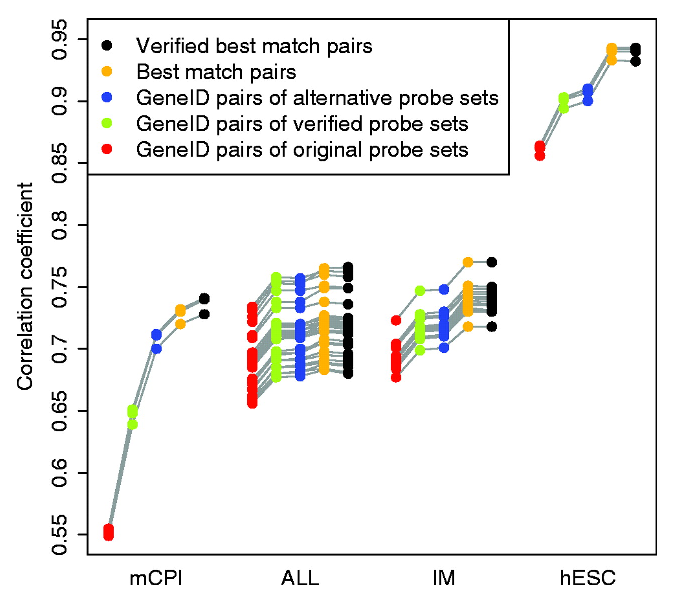
\includegraphics[width=.48\textwidth]{pic/gni.eps}}&
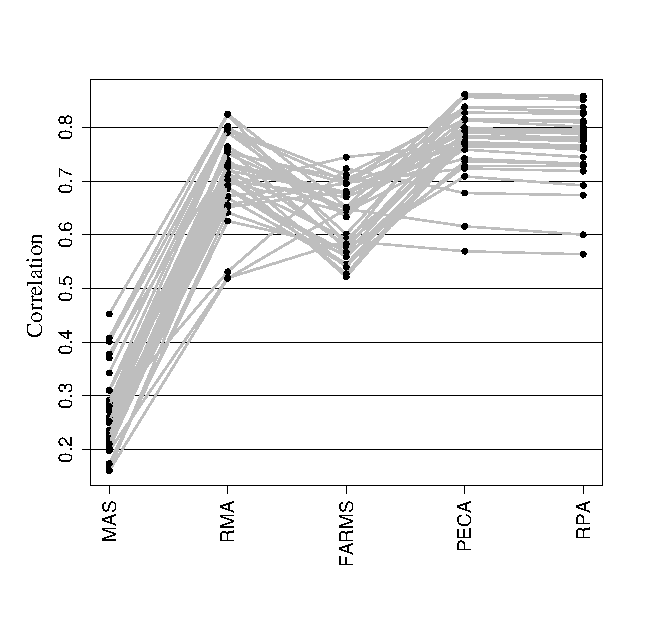
\includegraphics[width=.48\textwidth]{pic/ALLcomp-xfig.eps}
\end{tabular}
\caption{{\bf A} Effect of sequence verification on comparability
  between microarray platforms. Correlations between RMA-preprocessed
  technical replicates on two array platforms where the same samples
  have been hybridized on the two array types. The Pearson
  correlations were calculated for each pair of arrays measuring the
  same biological sample. The gray lines show correlations obtained
  with the different probe matching criteria. In the hESC array
  comparison, the best match probe sets contained exactly the same
  probes on both array generations, which resulted in very high
  correlations. The advantages of probe verification and alternative
  mappings were largest when arrays with different probe collections
  were compared in the mCPI, ALL and IM array comparisons. {\bf B}
  Reproducibility of signal estimates in real data sets between the
  technical replicates, i.e., the 'best match' probe sets between the
  HG-U95Av2 and HG-U133A platforms.  The consistency was measured by
  the Pearson correlation between the pairs of arrays, to which the
  same sample was hybridized. \copyright Published by Oxford
  University Press. Reprinted with permission from
  Publication~\ref{PECA}.}
\end{figure}

\section{Model-based noise reduction}\label{sec:modelnoise}

Standard approaches for investigating probe performance typically rely
on external information, such as genomic sequence data (see
\citealt{Mecham04b, Zhang05} and Publication~\ref{PECA}) or physical
models \citep{Naef03,Wu05}. However, such models cannot reveal probes
with uncharacterized sources of contamination, such as
cross-hybridization with alternatively spliced transcripts or closely
related mRNA sequences.  Vast collections of microarray data are
available in public repositories. These large-scale data sets contain
valuable information of both biological and technical aspects of gene
expression studies. Publication~\ref{RPA} introduces a data-driven
strategy to extract and utilize probe-level information in microarray
data collections.

The model, {\it Robust Probabilistic Averaging (RPA)}, is a
probabilistic preprocessing procedure that is based on explicit
modeling assumptions to analyze probe reliability and quantify the
uncertainty in measurement data based on gene expression data
collections, independently of external information of the probes. The
model can be viewed as a probabilistic extension of the probe-level
preprocessing approach for differential gene expression studies
presented in Publication~\ref{PECA}.  The explicit Bayesian
formulation quantifies the uncertainty in the model parameters, and
allows the incorporation of prior information concerning probe
reliability into the analysis. RPA provides estimates of probe
reliability, and a probeset-level estimate of differential gene
expression directly from expression data and independently of the
noise source. The RPA model is independent of physical models or
external and constantly updated information such as genomic sequence
data, but provides a framework for incorporating such prior
information of the probes in gene expression analysis.

Other probabilistic methods for microarray preprocessing include BGX
\citep{Hein05}, gMOS \citep{Milo03} and its extensions
\citep{Liu05}. The key difference to the RPA procedure of
Publication~\ref{RPA} is that these methods are designed to provide
probeset-level summaries of absolute gene expression levels, and
suffer from the same unidentifiability problem of probe affinity
parameters as the RMA algorithm \citep{Irizarry03rma}. In contrast,
RPA models probe-level estimates of differential gene expression. This
removes the unidentifiability issue, which is advantageous when the
objective is to compare gene expression levels between experimental
conditions. Another important difference is that the other
preprocessing methods do not provide explicit estimates of
probe-specific parameters, or tools to investigate probe performance.
Publication~\ref{RPA} assigns an explicit probabilistic measure of
reliability to each probe. This gives tools to analyze probe
performance and to guide probe design.


\subsubsection{Robust Probabilistic Averaging}

Let us now consider in more detail the probabilistic preprocessing
framework, RPA, introduced in Publication~\ref{RPA}. Probe performance
is ultimately determined by its ability to accurately measure the
expression level of the target transcript, which is unknown in
practical situations.  Although the performance of individual probes
varies, the collection of probes designed to measure the same
transcript will provide ground truth for assessing probe performance
(Figure~\ref{fig:badprobe}A). RPA captures the shared signal of the
probes within a probeset, and assumes that the shared signal
characterizes the expression of the common target transcript of the
probes. The reliability of individual probes is estimated with respect
to the strongest shared signal of the probes. RPA assumes normally
distributed probe effects, and quantifies probe reliability based on
probe variance around the probeset-level signal across a large number
of arrays. This extends the formulation of the RMA model in
Equation~\ref{eq:rmamodel} by introducing an additional probe-specific
Gaussian noise component:

\begin{equation}\label{eq:rpa}
  \sij = \gi + \muj + \epsilonij.
\end{equation}

\noindent In contrast to RMA, the variance is probe-specific in this
model, and distributed as \(\epsilonij \sim N(0,\taujSq)\). The
variance parameters \(\taus\) are of interest in probe reliability
analysis; they reflect the noise level of the probe, in contrast to
probe-level preprocessing methods that focus on estimating the
unidentifiable mean parameter of the Gaussian noise model,
corresponding to probe affinity \citep[see e.g.][]{Irizarry03rma,
  Li01mbei}. In Publication~\ref{RPA}, probe-level calculation of
differential expression avoids the need to model unidentifiable probe
affinities, the key probe-specific parameter in other probe-level
preprocessing methods. More formally, the unidentifiable probe
affinity parameters \(\mu_.\) cancel out in RPA when the signal
log-ratio between a user-specified 'reference' array and the remaining
arrays is computed for each probe: the differential expression signal
between arrays \(t = \{1, \dots, T\} \) and the reference array \(c\)
for probe \(j\) is obtained by \(\mtj = \stj - \scj = \gt - \gc +
\epsilontj - \epsiloncj = \dt + \epsilontj - \epsiloncj\). In vector
notation, the differential expression profile of probe \(j\) across
the \(T\) arrays is then written as \(\mj = \d + \Epsilonj\), i.e.,
a noisy observation of the true underlying differential expression
signal \(\d\) and probe-specific noise \(\Epsilonj\).


The unidentifiable probe affinity parameters cancel out in the RPA
model of Publication~\ref{RPA}. This can partly explain the previous
empirical observations that calculating differential expression
already at probe-level improves the analysis of differential gene
expression \citep{Zhang02, Elo05}. However, the previous models are
non-probabilistic preprocessing methods that do not aim at quantifying
the uncertainty in the probes. Use of a single parameter for probe
effects in RPA also gives more straightforward interpretations of
probe reliability.

Posterior estimates of the model parameters are derived to estimate
probe reliability and differential gene expression. The differential
expression vector \(\d = \{d_t\}\) and the probe-specific variances
\(\TauSq = \{\taujSq\}\) are estimated simultaneously.  The posterior
density of the model parameters is obtained from the likelihood of the
data and the prior according to Bayes' rule
(Equation~\ref{eq:bayesrule}) as

\begin{equation}\label{eq:rpapost1}
    p(\d, \TauSq | \m) \sim p(\m | \d, \TauSq) p(\d, \TauSq).
\end{equation}

\noindent To obtain this posterior, let us consider the likelihood
\(p(\m | \d, \TauSq)\) of the data and the prior \(p(\d, \TauSq)\) of the
model parameters. The noise on the selected control array
\(\epsiloncj\) is a latent variable, and marginalized out in the model
to obtain the likelihood:

\begin{equation}
\begin{split}
p(\m | \d, \TauSq) 
= \prod_{tj} \int N(\mtj | \dt - \epsiloncj, \taujSq) N(\epsiloncj | 0, \taujSq) d\epsiloncj \\
\sim \prod_j (2 \pi \taujSq)^{-\frac{T}{2}} exp(- \frac{\sum_t (\mtj -\dt)^2 - \frac{ [\sum_t (\mtj - \dt)]^2} {T + 1}}{2 \taujSq}).
\end{split}
\label{eq:datalikelihood}
\end{equation}

\noindent Let us assume independent priors, \(p(\d,\TauSq) = p(\d)
p(\TauSq)\), flat non-informative prior \(p(\d) \sim 1\) and
conjugate priors for the variance parameters in \(\TauSq\) (inverse
Gamma function, see \citealt{Gelman03}). With these standard
assumptions, the prior takes the form

\begin{equation}\label{eq:rpaprior}
  p(\d,\TauSq) \sim \prod_j IG(\taujSq; \alphaj, \betaj),
\end{equation}

\noindent where \(\alphaj\) and \(\betaj\) are the shape and scale parameters of
the inverse Gamma distribution. Prior information of the probes can be
incorporated in the analysis through these parameters. Probe-level
differential expression is then described by two sets of parameters;
the differential gene expression vector \(\d = [d_1 \dots d_T]\), and
the probe-specific variances \(\TauSq = [\tau^2_1 \dots \tau^2_J]\).
High variance \(\taujSq\) indicates that the probe-level observation
\(\mj\) is strongly deviated from the estimated true signal
\(\d\). Denoting \(\alphahatj = \alphaj + \frac{T}{2}\) and
\(\betahatj = \betaj + \frac{1}{2}\sum_t (\mtj - \dt)^2 -
\frac{1}{2}\frac{(\sum_t (\mtj - \dt))^2}{T+1}\), the posterior of the
model parameters in Equation~\ref{eq:rpapost1} takes the form

\begin{equation}
\label{eq:fullpost}
p(\d, \TauSq | \m) \sim \prod_j (\taujSq)^{-(\alphahatj + 1)} exp(-\frac{\betahatj}{\taujSq}).
\end{equation}

\noindent The formulation allows estimating the uncertainty in the
expression estimates and probe-level parameters.  In practice, a MAP
point estimate of the parameters, obtained by maximizing the
posterior, is often sufficient. In the limit of a large sample size
(\(T \rightarrow \infty\)), the model will converge to estimating
ordinary mean and variance parameters. With limited sample sizes that
are typical in microarray studies the prior parameters provide
regularization that makes the probabilistic formulation more robust to
overfitting and local optima, compared to direct estimation of the
mean and variance parameters. Moreover, the probabilistic analysis
takes the uncertainty in the data and model parameters into account in
an explicit manner.

The model also provides a principled framework for incorporating prior
knowledge probe reliability in microarray preprocessing through the
probe-specific hyperparameters \(\alpha, \beta\). Estimation and use
of probe-specific effects from external microarray data collections
has been previously suggested in the context of the refRMA method by
\cite{Katz06}, where such side information was shown to improve gene
expression estimates. The RPA method of Publication~\ref{RPA} provides
an alternative probabilistic treatment.

\subsubsection{Model validation}

The probabilistic RPA model introduced in Publication~\ref{RPA} was
validated by comparing the preprocessing performance to other
preprocessing methods, and additionally by comparing the estimates of
probe-level noise to known sources of probe-level contamination.  The
comparison methods include the FARMS \citep{Hochreiter06}, MAS5
\citep{Hubbell2002}, PECA (Publication~\ref{PECA}), and RMA
\citep{Irizarry03rma} preprocessing algorithms. FARMS has a more
detailed model for probe effects than the other methods, and it
contains implicitly a similar probe-specific variance parameter than
our RPA model. FARMS is based on a factor analysis model, and is
defined as \(\sij = z_i \lambdaj + \muj + \epsilonij\), where \(z_i\)
captures the underlying gene expression. In contrast to RMA and RPA
that have a single probe-specific parameter, FARMS has three
probe-specific parameters \(\{\lambdaj, \muj, \epsilonij\}\). MAS5 is
a standard preprocessing algorithm provided by the array
manufacturer. The algorithm performs local background correction,
utilizes so-called mismatch probes to control for non-specific
hybridization, and scales the data from each array to the same average
intensity level to improve comparability across arrays. MAS5
summarizes probe-level observations of absolute gene expression levels
using robust summary statistics, Tukey biweight estimate, but unlike
FARMS, RMA and RPA, MAS5 does not model probe-specific effects.

The preprocessing performance of these methods was investigated in
spike-in experiments where certain target transcripts measured by the
array have been spiked in at known concentrations, as well as on real
data sets.  The results from the spike-in experiments were compared in
terms of receiver operating characteristics (ROC).  The standard RMA,
PECA (Publication~\ref{PECA}) and RPA (Publication~\ref{RPA}) had
comparable performance in spike-in data, and they outperformed the
MAS5 \citep{Hubbell2002} and FARMS \citep{Hochreiter06} preprocessing
algorithms in estimating differential gene expression. On real data
sets, PECA and RPA outperformed the other methods, providing higher
reproducibility between technical replicates measured on different
microarray platforms (Figure~\ref{fig:rpaReproducibility}B).

In contrast to standard preprocessing algorithms, RPA provides
explicit quantitative estimates of probe performance. The model has
been validated on widely used human whole-genome arrays by comparing
the estimates of probe reliability with known probe-level error
sources: errors in probe-genome alignment, interrogation position of a
probe on the target sequence, GC-content, and the presence of SNPs in
the probe target sequences; a good model for assessing probe
reliability should detect probes contaminated by the known error
sources.  The results from our analysis can be used to characterize
the relative contribution of different sources of probe-level noise
(Figure~\ref{fig:badprobe}B). In general, the probes with known sources
of contamination were more noisy than the other probes, with 7-39\%
increase in the average variance, as detected by RPA.  Any single
source of error seems to explain only a fraction of the most highly
contaminated probes. A large portion (35-60\%) of the detected least
reliable probes were not associated with the investigated known noise
sources. This suggests that previous methods that remove probe-level
noise based on external information, such as genomic alignments will
fail to detect a significant portion of poorly performing probes.  The
RPA model of Publication~\ref{RPA} provides rigorous algorithmic tools
to investigate the various probe-level error sources. Better
understanding of the factors affecting probe performance can advance
probe design and contribute to reducing probe-related noise in future
generations of gene expression arrays.

\section{Conclusion}\label{sec:preconclusion}

The contributions presented in this Chapter provide improved
preprocessing strategies for differential gene expression studies. The
introduced techniques utilize probe-level analysis, as well as side
information in sequence and microarray databases.  Probe-level studies
have led to the establishment of probe verification and alternative
microarray interpretations as a standard step in microarray
preprocessing and analysis. The alternative interpretations for
microarray data based on updated genomic sequence data
\citep{Gautier04b, Dai05} are now implemented as routine tools in
popular preprocessing algorithms such as the RMA, or the RPA method of
Publication~\ref{RPA}. The probe-level analysis strategy has been
recently extended to exon array context, where expression levels of
alternative splice variants of the same genes are compared under
particular experimental conditions. The probe-level approach has shown
superior preprocessing performance also with exon arrays
\citep{Laajala2009}.  A convenient access to the algorithmic tools
developed in Publications~\ref{PECA} and~\ref{RPA} for microarray
preprocessing and probe-level analysis is provided by the accompanied
open source implementation in
BioConductor.\footnote{http://www.bioconductor.org/packages/release/bioc/html/RPA.html}


